\section{Actor-Critique Pipeline}
\label{sec:actor-critique-results}

This section presents comprehensive experimental results for our actor-critique pipeline (Architecture 2), powered by Google Gemini 2.5 Flash. We evaluate the model's performance across five languages on the development set, analyzing both narrative and subnarrative classification effectiveness, cross-linguistic performance patterns, and detailed error characteristics through confusion matrix analysis.

\subsection{Experimental setup and evaluation framework}

Our evaluation was conducted on the multilingual development set comprising 178 documents across five languages: Bulgarian (BG, 35 files), English (EN, 41 files), Hindi (HI, 35 files), Portuguese (PT, 35 files), and Russian (RU, 32 files). The actor-critique pipeline employs a two-stage validation process where an initial classification agent provides predictions, followed by a critique agent that validates and refines these predictions. This architecture aims to address the error propagation and semantic ambiguity limitations identified in the zero-shot agentic framework.

Our primary evaluation metrics are F1 Coarse (for narratives) and F1 Sample (for subnarratives), providing balanced assessment of multi-label performance at both hierarchical levels by evaluating each document's label set independently.

\subsection{Overall multilingual performance analysis}

Figure~\ref{fig:actor-critique-language-performance} presents the overall performance comparison across languages, revealing significant cross-linguistic performance variations.

\begin{figure}[htbp]
    \centering
    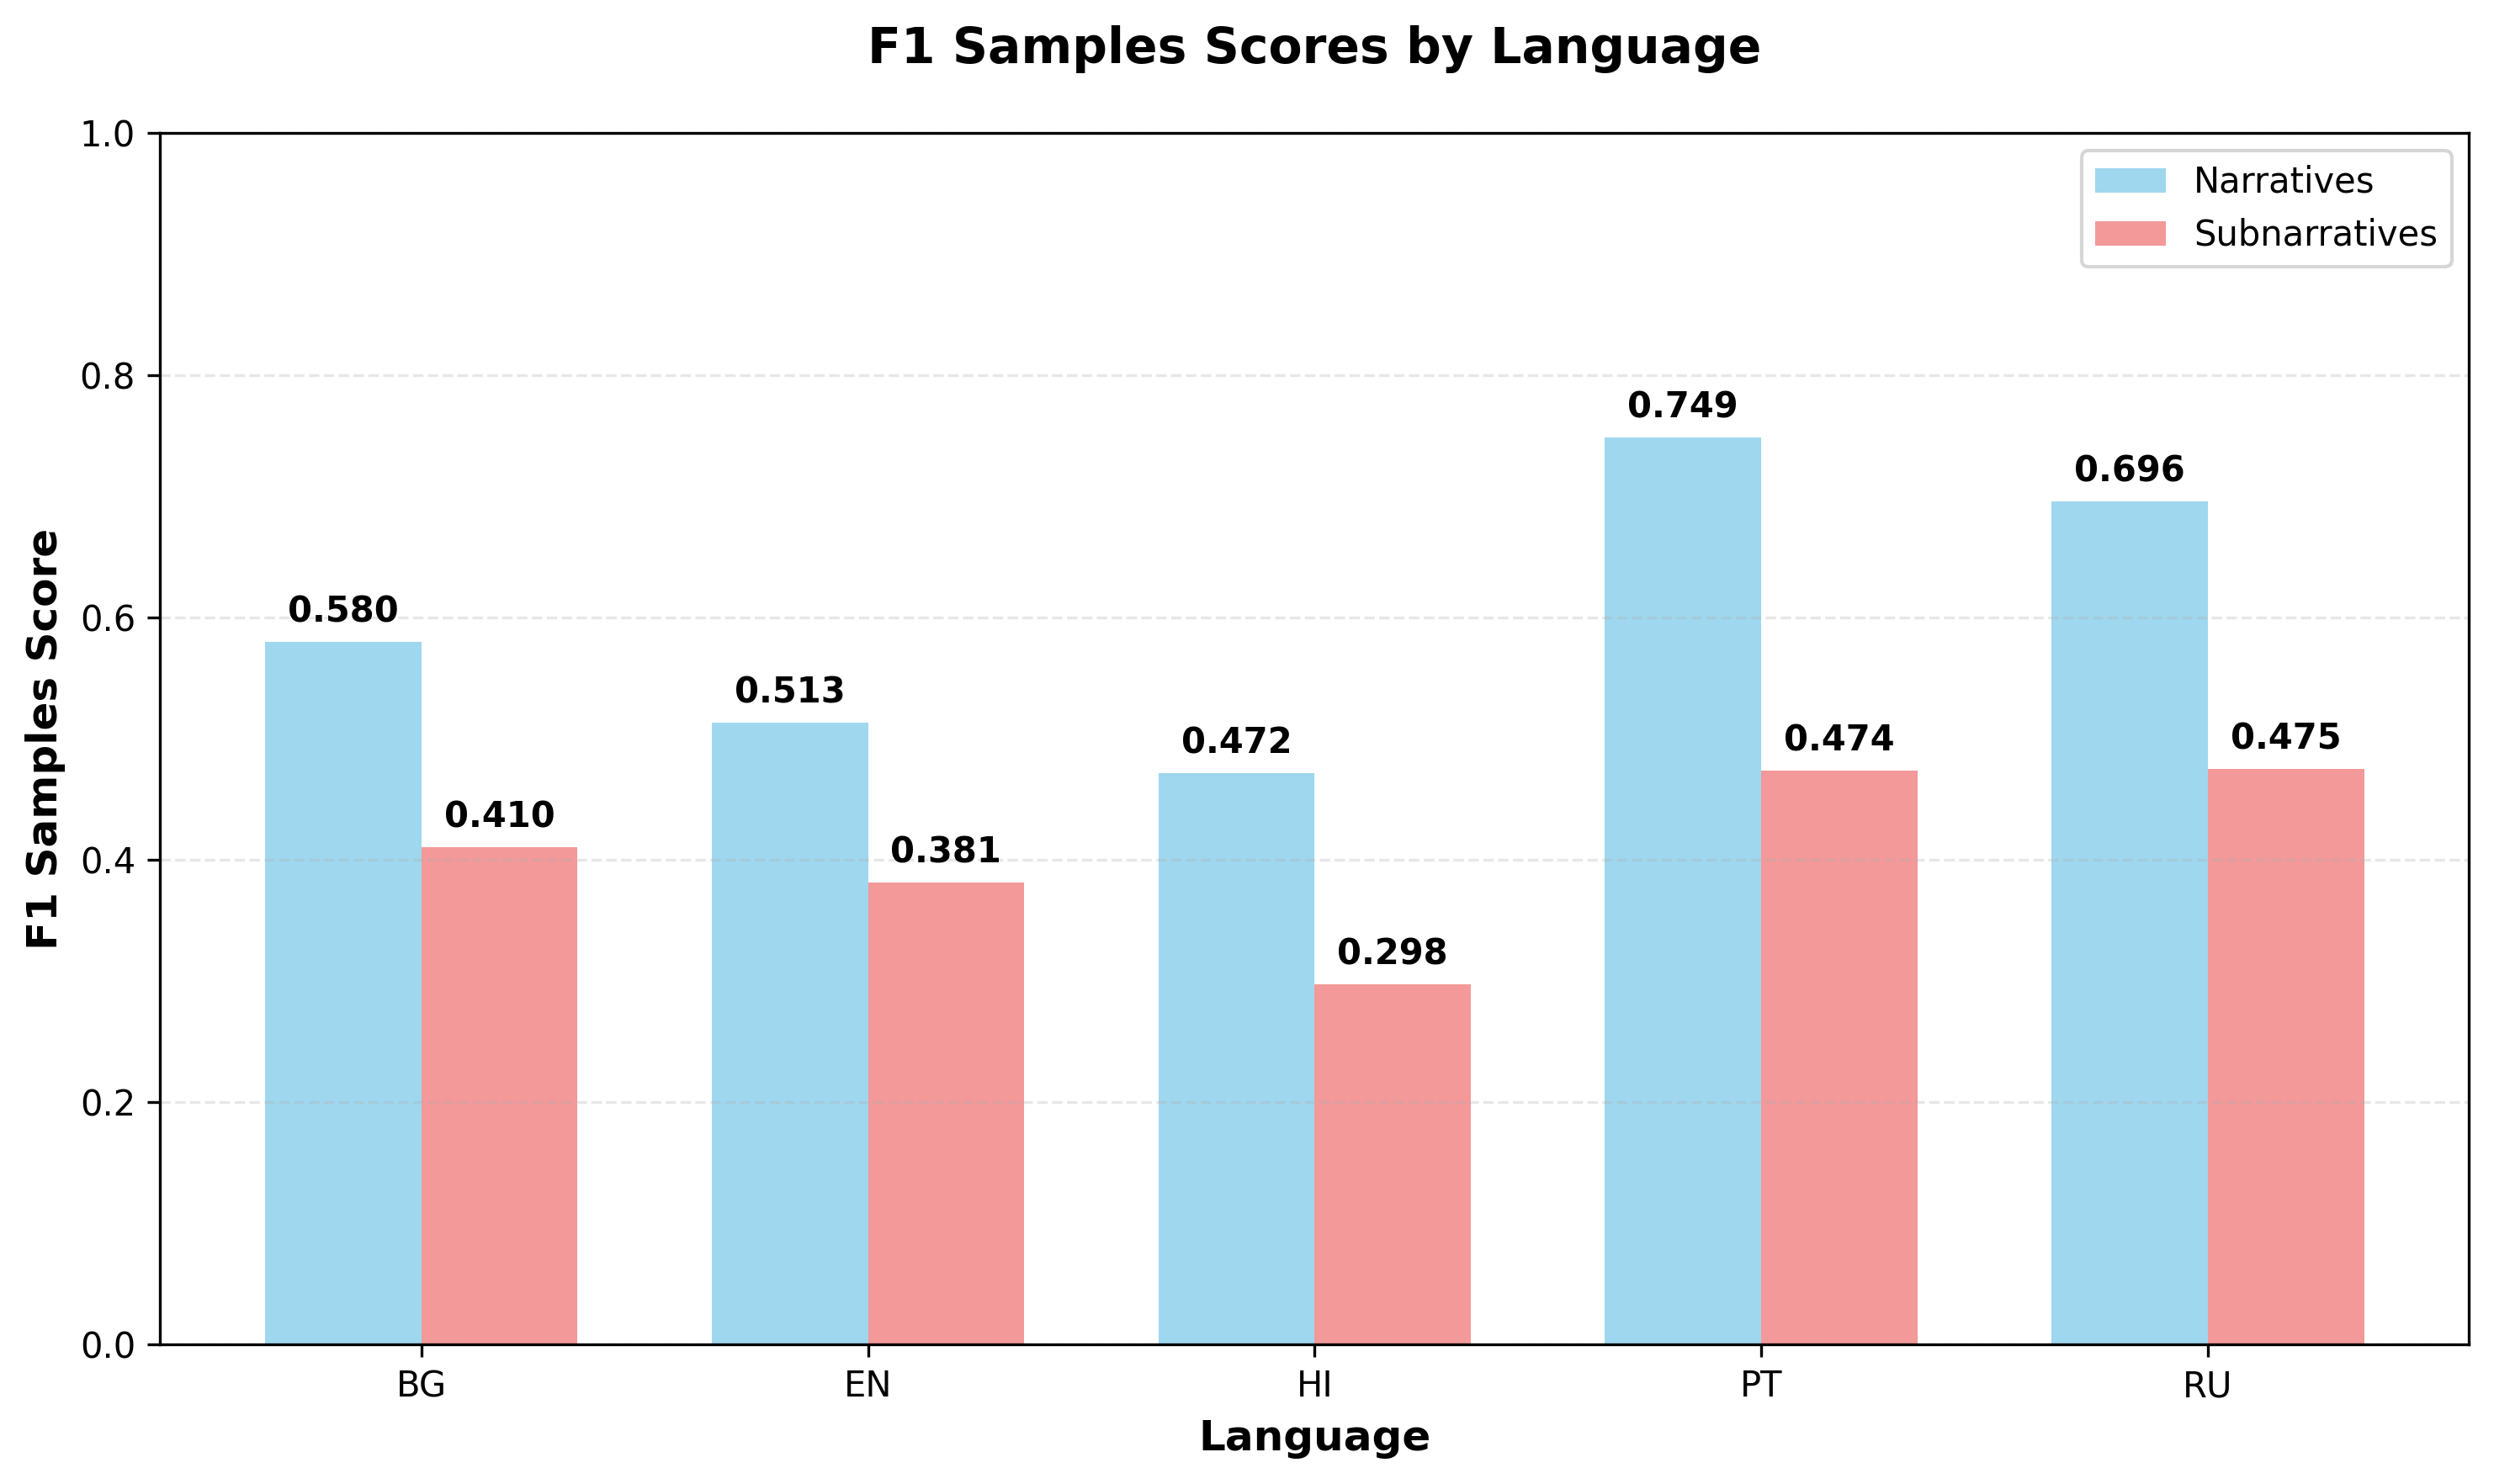
\includegraphics[width=0.8\textwidth]{gemini25_flash_devset_evaluation/plots/f1_samples_by_language.png}
    \caption{F1 Samples performance by language, highlighting Portuguese as the best-performing language and revealing the substantial performance gap between high-resource (PT, RU) and low-resource (HI) languages.}
    \label{fig:actor-critique-language-performance}
\end{figure}

\begin{table}[htbp]
\centering
\caption{Actor-Critique Pipeline performance across languages on the development set. Columns report F1 Coarse (narratives) and F1 Sample (subnarratives).}
\label{tab:actor-critique-performance}
\begin{tabular}{lccc}
	\toprule
	\textbf{Language} & \textbf{Files} & \textbf{F1 Coarse} & \textbf{F1 Sample} \\
\midrule
	\textbf{Portuguese (PT)} & 35 & \textbf{0.7489} & \textbf{0.4737} \\
	\textbf{Russian (RU)} & 32 & 0.6958 & 0.4754 \\
	\textbf{Bulgarian (BG)} & 35 & 0.5799 & 0.4104 \\
	\textbf{English (EN)} & 41 & 0.5132 & 0.3815 \\
	\textbf{Hindi (HI)} & 35 & 0.4715 & 0.2976 \\
\midrule
	\textbf{Average} & -- & \textbf{0.6019} & \textbf{0.4077} \\
\bottomrule
\end{tabular}
\end{table}

\paragraph{Portuguese demonstrates exceptional performance.} Portuguese achieves the highest F1 Coarse for narratives (0.7489) and the highest F1 Sample for subnarratives (0.4737), establishing a 59\% performance advantage over the lowest-performing language (Hindi). This exceptional performance suggests that the actor-critique pipeline effectively leverages the cultural and linguistic patterns present in Portuguese text.

\paragraph{Strong Russian performance validates multilingual capabilities.} Russian achieves the second-highest F1 Coarse for narratives (0.6958) and strong F1 Sample for subnarratives (0.4754), demonstrating that the pipeline successfully handles Cyrillic script and Russian linguistic structures.

\paragraph{Hindi presents systematic challenges.} Hindi shows the most substantial performance degradation across all metrics, with particularly poor subnarrative performance (F1 Sample: 0.2976). This 37\% gap compared to Portuguese subnarratives suggests systematic challenges in processing Hindi text within the current pipeline architecture.

\subsection{Hierarchical performance characteristics}

The actor-critique pipeline demonstrates a consistent pattern of performance degradation from narrative to subnarrative classification across all languages:

\begin{itemize}
    \item \textbf{Average performance gap}: 19.4\% reduction from F1 Coarse (narratives, 0.6019) to F1 Sample (subnarratives, 0.4077).
    \item \textbf{Smallest gap}: English (13.2\% reduction).
    \item \textbf{Largest gap}: Portuguese (27.4\% reduction).
\end{itemize}

This hierarchical performance pattern is significantly smaller than observed in the transformer baseline (60\% reduction), suggesting that the actor-critique validation process effectively mitigates some error propagation issues inherent in hierarchical classification.

\subsection{Language-specific narrative performance analysis}

Figure~\ref{fig:narrative-performance-by-language} illustrates the top-performing narrative categories for each language, revealing distinct cross-linguistic patterns.

\begin{figure}[htbp]
    \centering
    \begin{subfigure}[b]{0.32\textwidth}
        \centering
        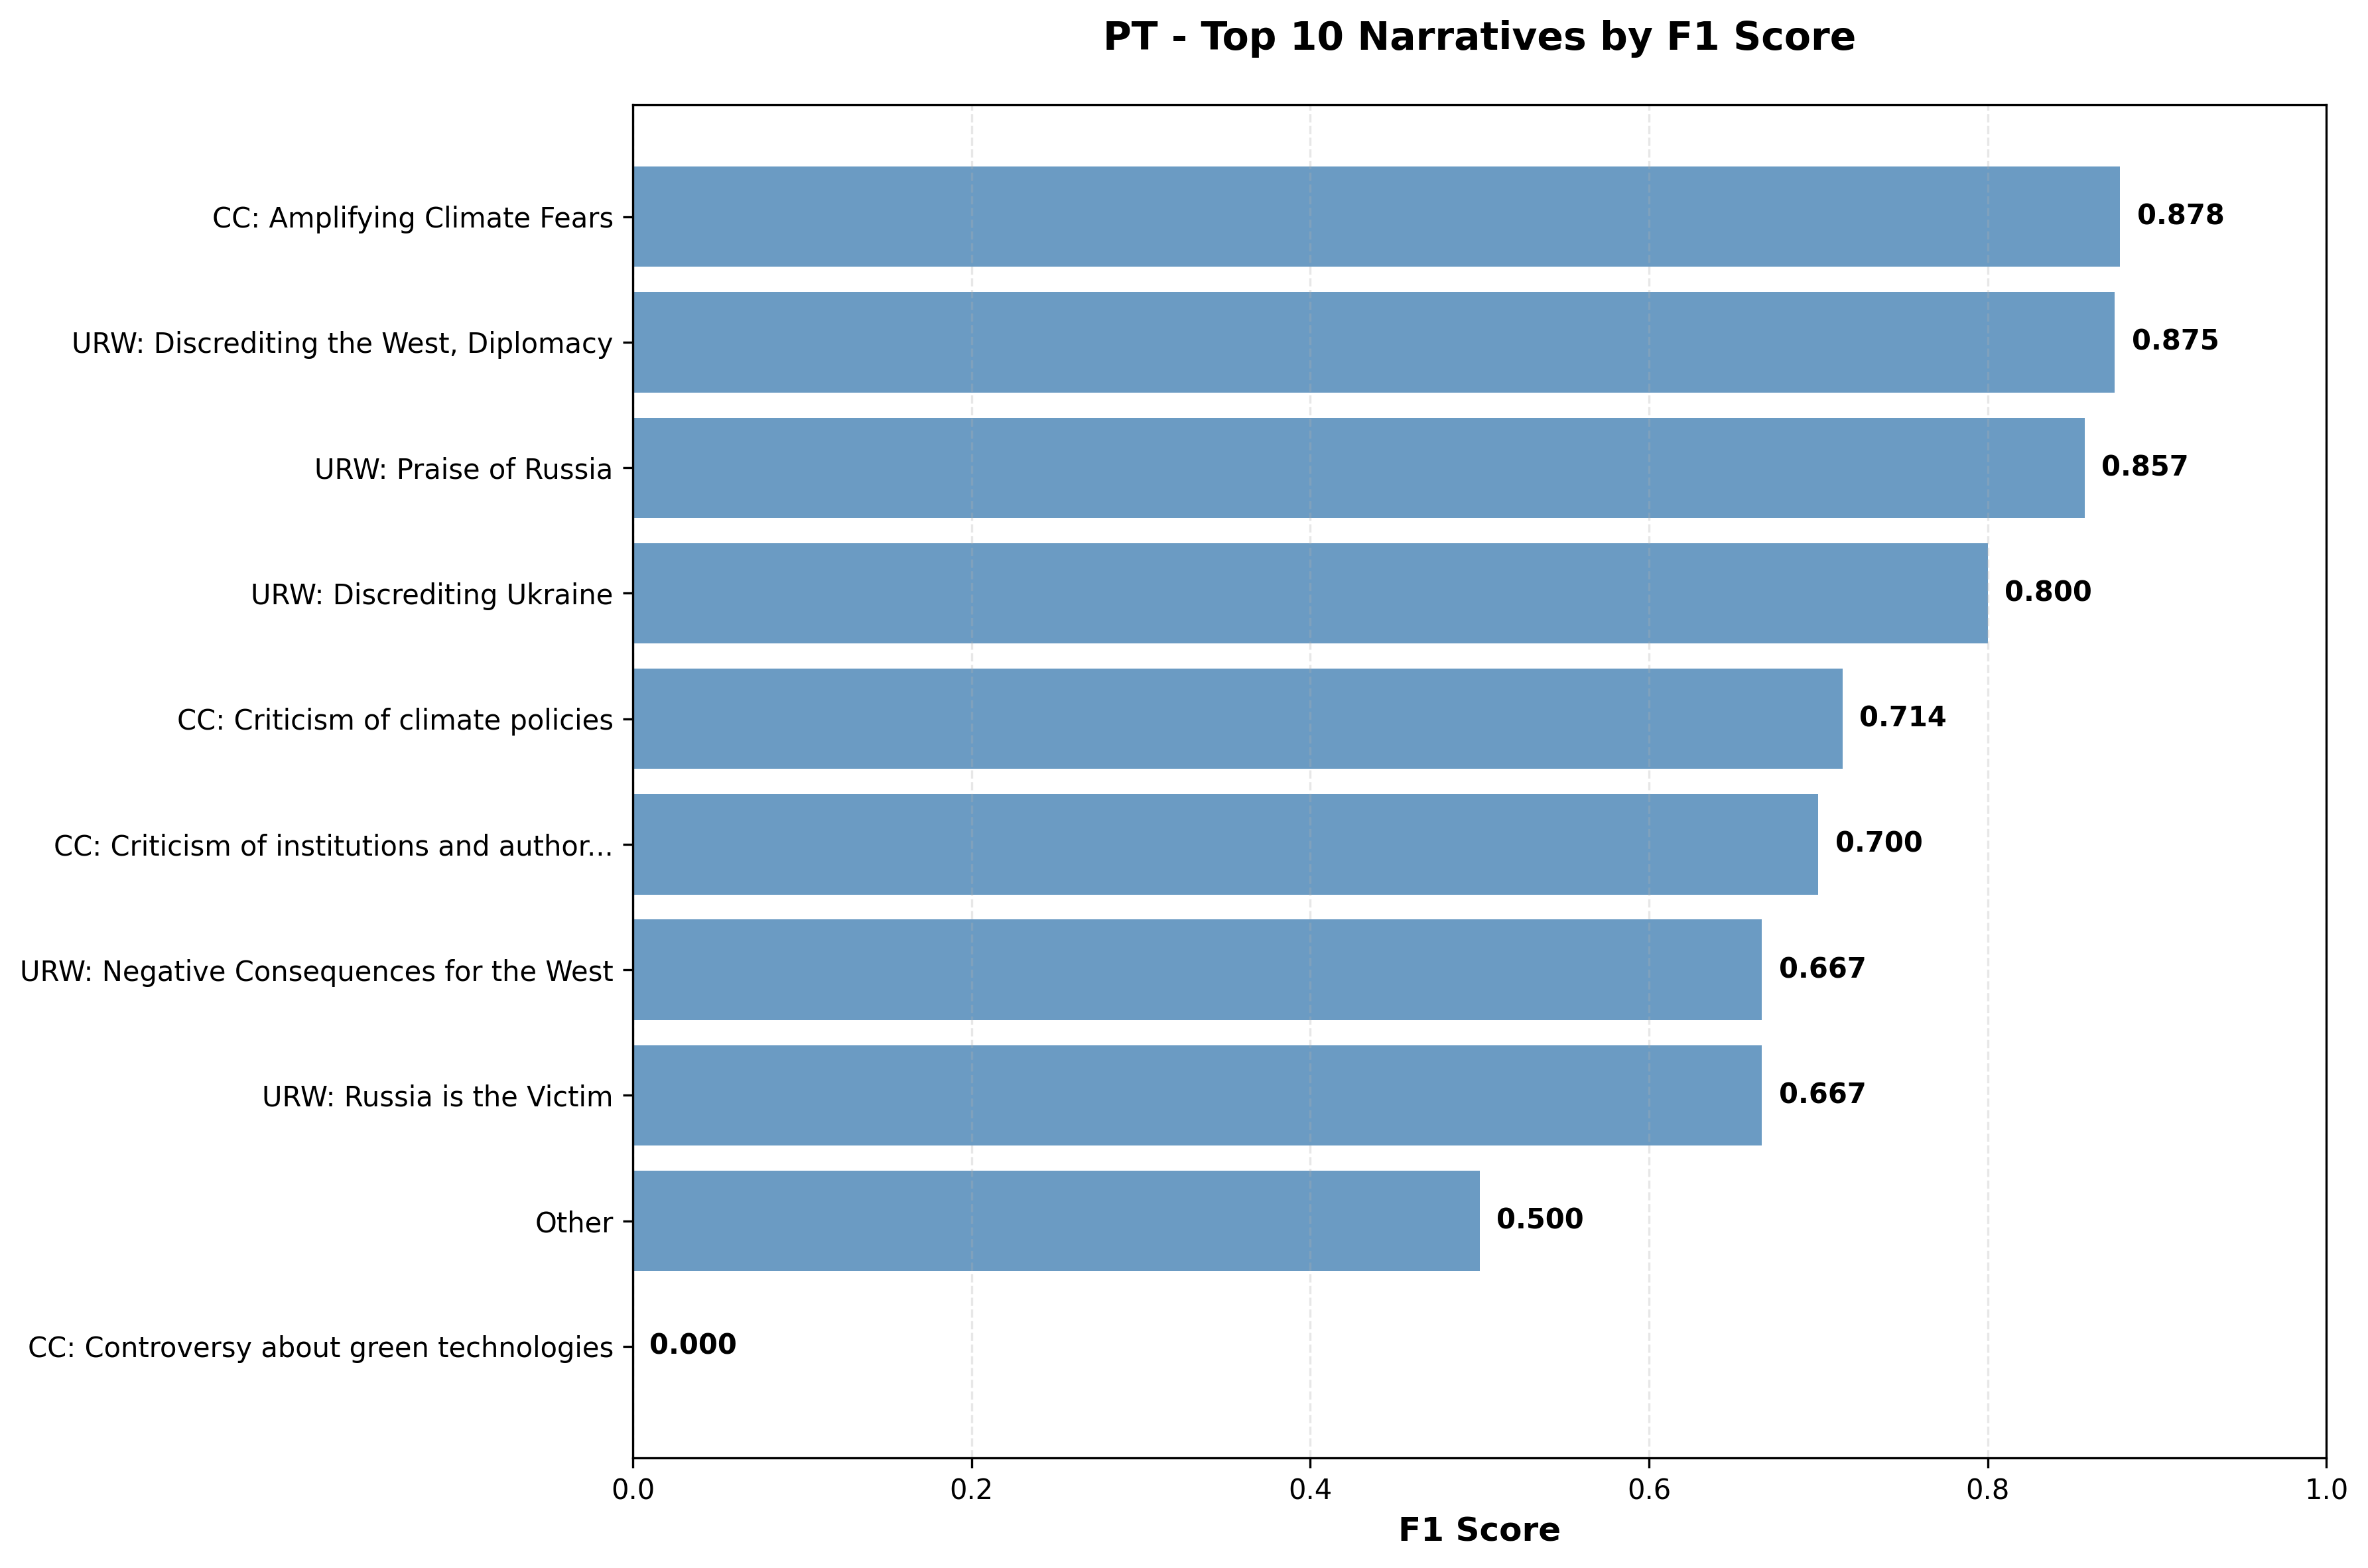
\includegraphics[width=\textwidth]{gemini25_flash_devset_evaluation/plots/PT_top_narratives_f1_scores.png}
        \caption{Portuguese narratives}
        \label{fig:pt-narratives}
    \end{subfigure}
    \hfill
    \begin{subfigure}[b]{0.32\textwidth}
        \centering
        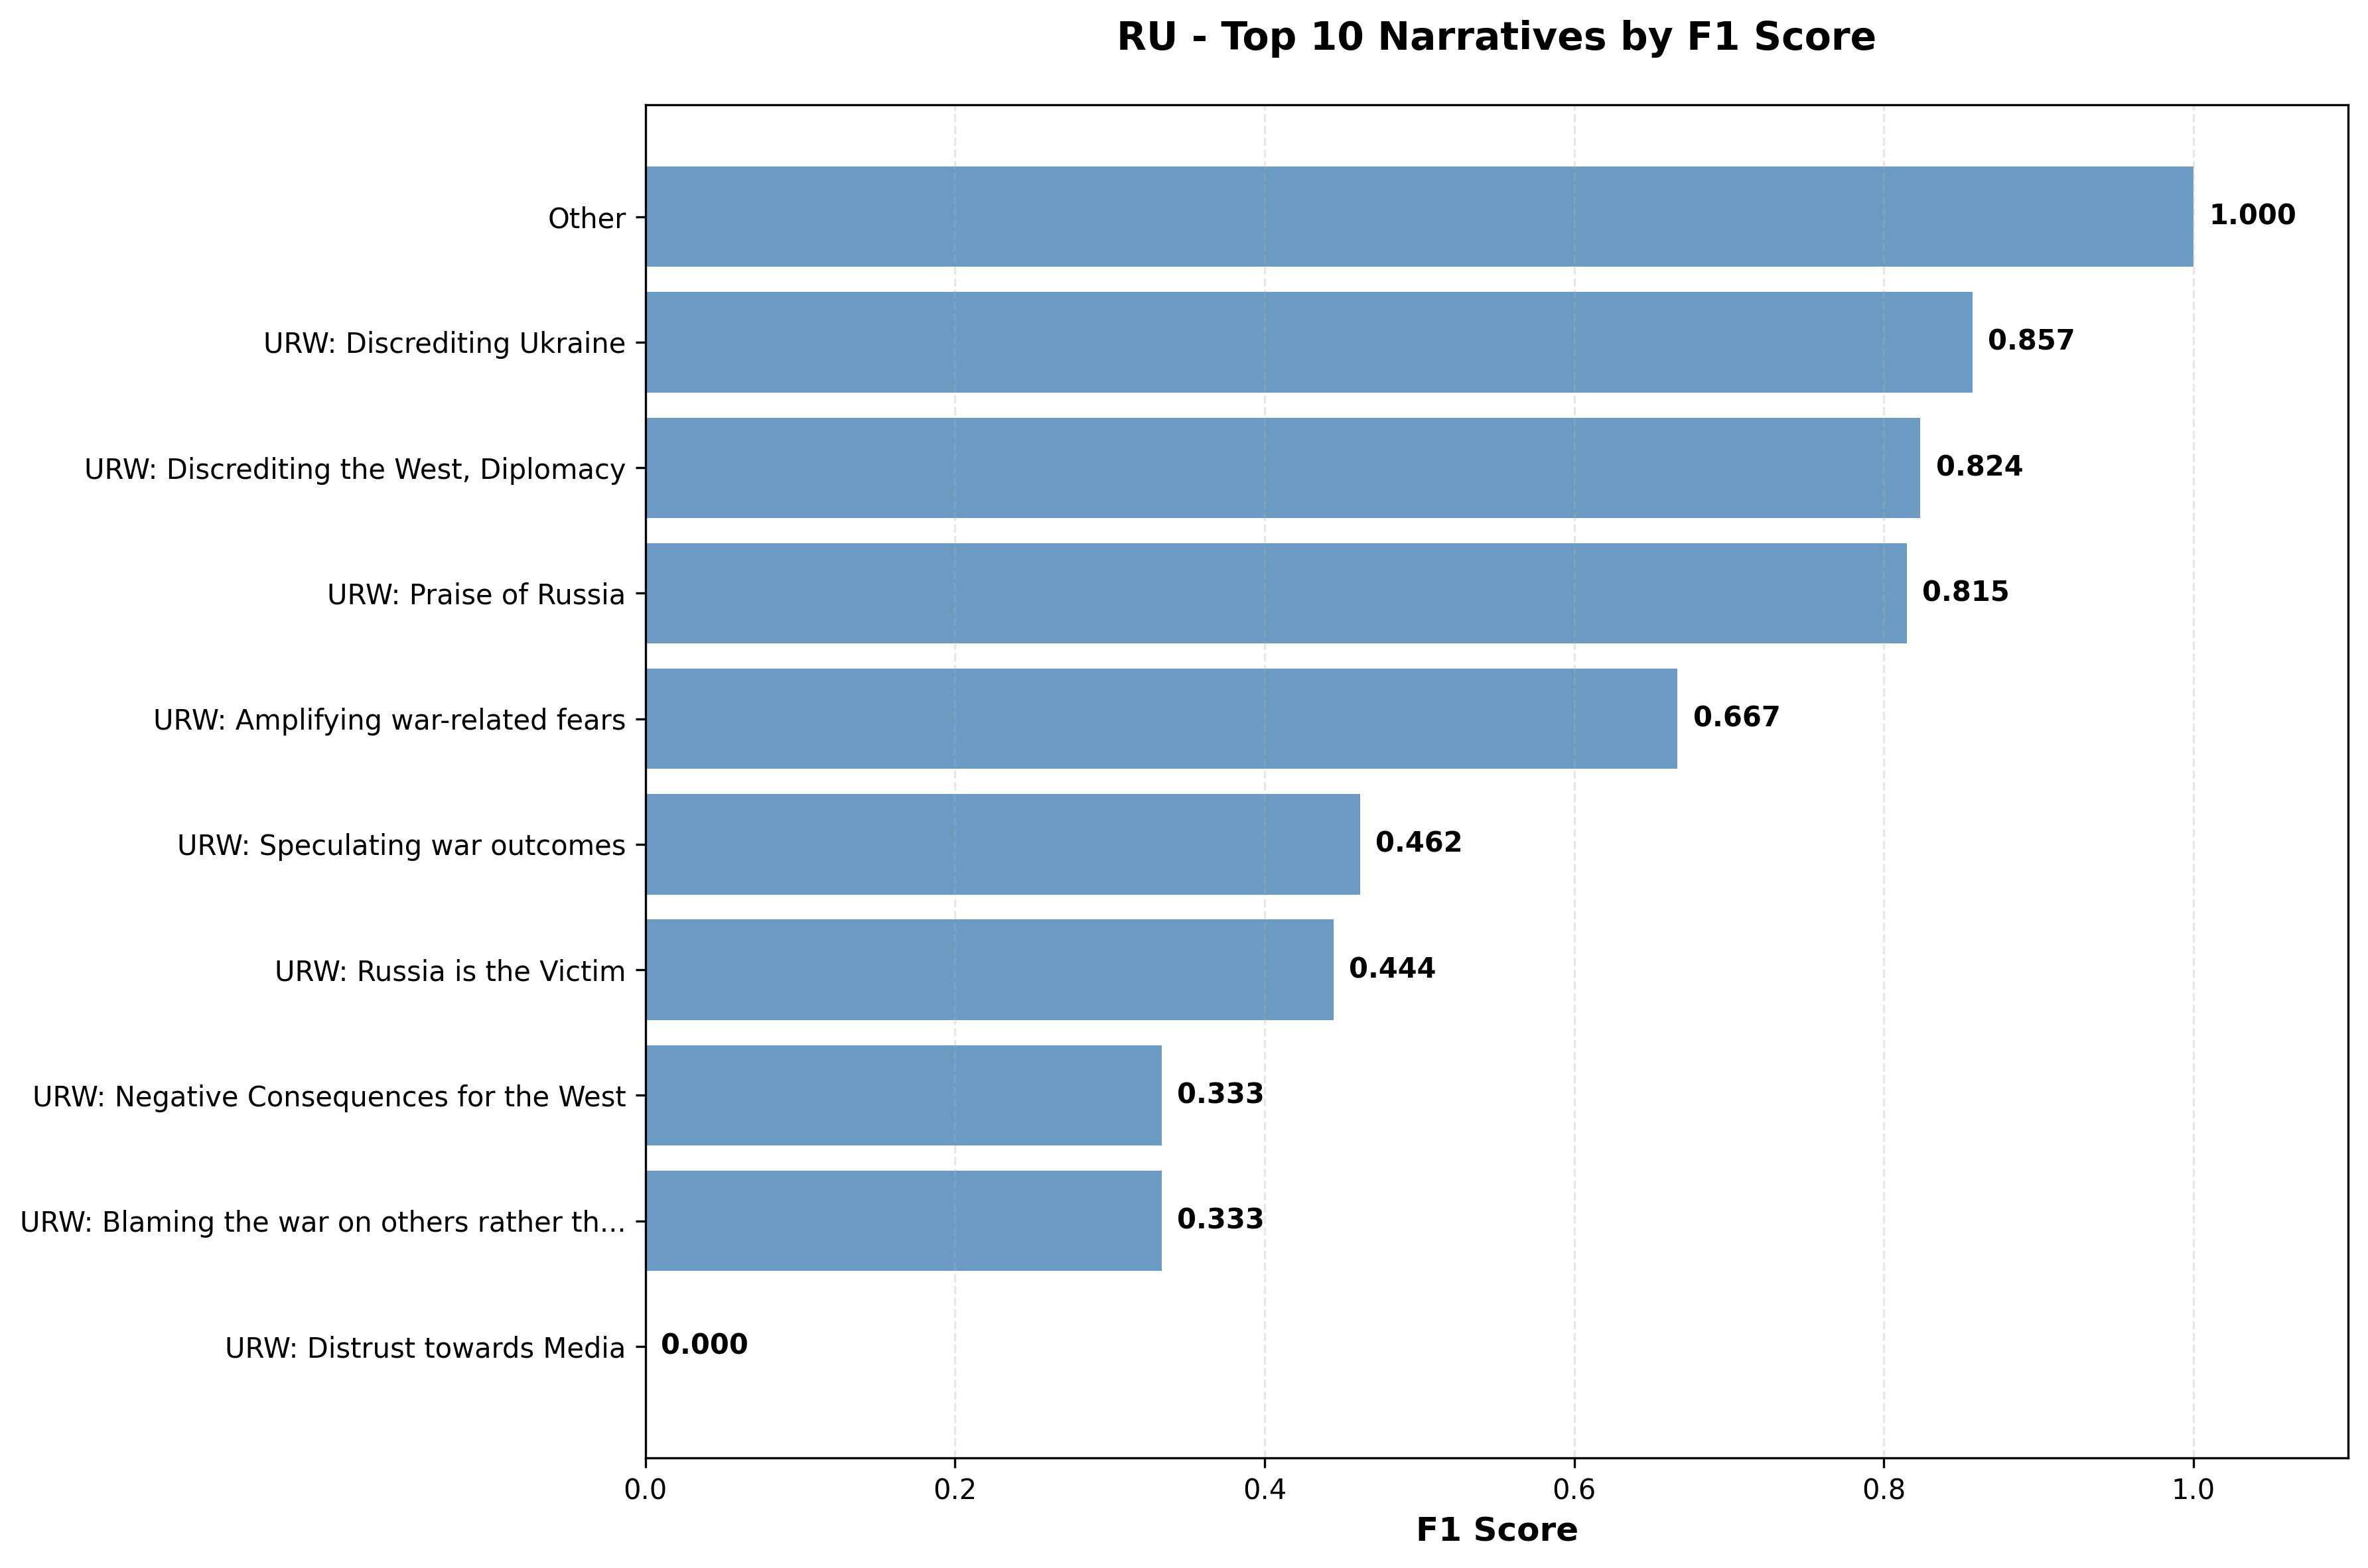
\includegraphics[width=\textwidth]{gemini25_flash_devset_evaluation/plots/RU_top_narratives_f1_scores.png}
        \caption{Russian narratives}
        \label{fig:ru-narratives}
    \end{subfigure}
    \hfill
    \begin{subfigure}[b]{0.32\textwidth}
        \centering
        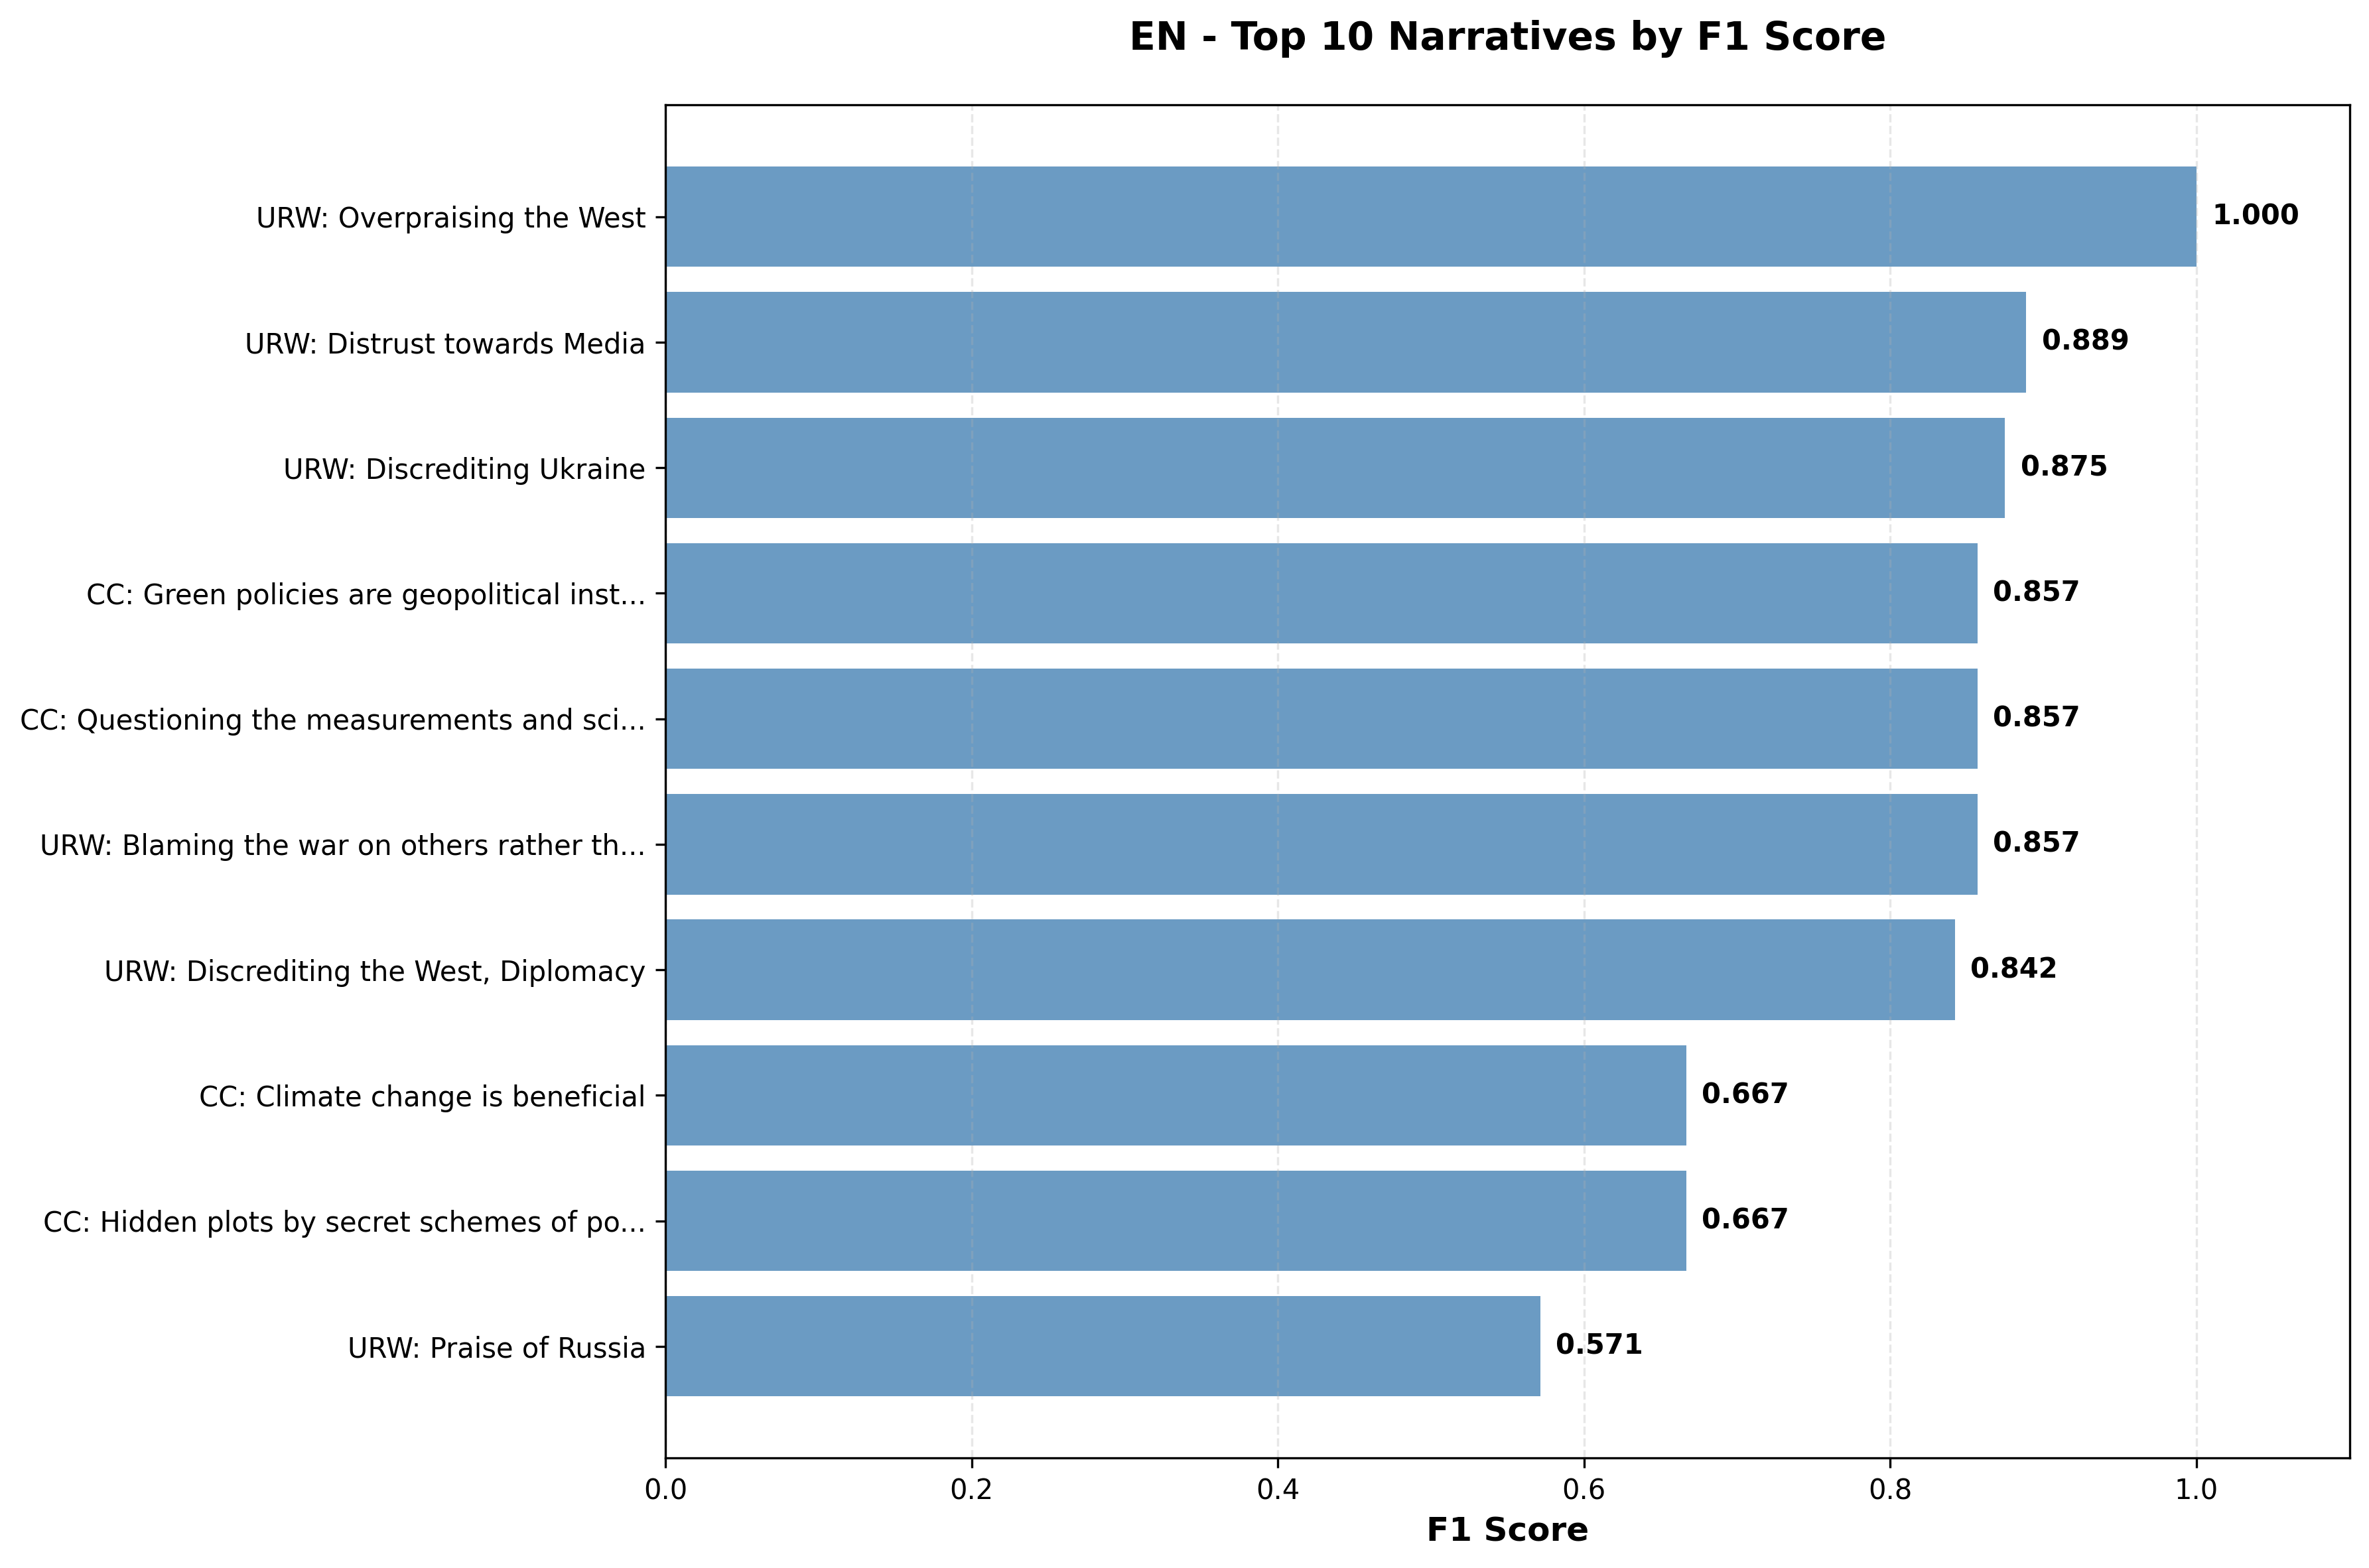
\includegraphics[width=\textwidth]{gemini25_flash_devset_evaluation/plots/EN_top_narratives_f1_scores.png}
        \caption{English narratives}
        \label{fig:en-narratives}
    \end{subfigure}
    \caption{Top-performing narrative categories by language, showing the actor-critique pipeline's effectiveness varies significantly across narrative types and languages. Portuguese and Russian show strong performance on climate and war narratives respectively, while English demonstrates more balanced performance across categories.}
    \label{fig:narrative-performance-by-language}
\end{figure}

\subsubsection{Portuguese narrative excellence}

Portuguese demonstrates exceptional performance across climate change narratives:
\begin{itemize}
    \item \textbf{CC: Amplifying Climate Fears}: F1 = 0.878 (perfect precision: 1.000)
    \item \textbf{URW: Discrediting the West, Diplomacy}: F1 = 0.875 
    \item \textbf{URW: Praise of Russia}: F1 = 0.857 (perfect precision: 1.000)
\end{itemize}

The consistently high precision scores (many achieving 1.000) indicate that the Portuguese language processing benefits significantly from the actor-critique validation mechanism, effectively eliminating false positives.

\subsubsection{Russian war narrative specialization}

Russian text shows particular strength in war-related narratives:
\begin{itemize}
    \item \textbf{Other}: Perfect performance (F1 = 1.000)
    \item \textbf{URW: Discrediting Ukraine}: F1 = 0.857 with high recall (1.000)
    \item \textbf{URW: Discrediting the West, Diplomacy}: F1 = 0.824
    \item \textbf{URW: Praise of Russia}: F1 = 0.815 with high precision (0.917)
\end{itemize}

This pattern suggests that the pipeline effectively captures Russian-specific linguistic markers for war-related propaganda narratives.

\subsubsection{English balanced performance}

English demonstrates more balanced performance across both climate and war narratives:
\begin{itemize}
    \item Multiple perfect scores on specific categories (F1 = 1.000)
    \item Strong performance on technical climate narratives (CC: Questioning measurements and science: F1 = 0.857)
    \item Effective war narrative detection (URW: Discrediting Ukraine: F1 = 0.875)
\end{itemize}

\subsection{Subnarrative classification analysis}

Figure~\ref{fig:subnarrative-performance-by-language} presents the fine-grained classification performance, highlighting the challenges of semantic disambiguation at the subnarrative level.

\begin{figure}[htbp]
    \centering
    \begin{subfigure}[b]{0.48\textwidth}
        \centering
        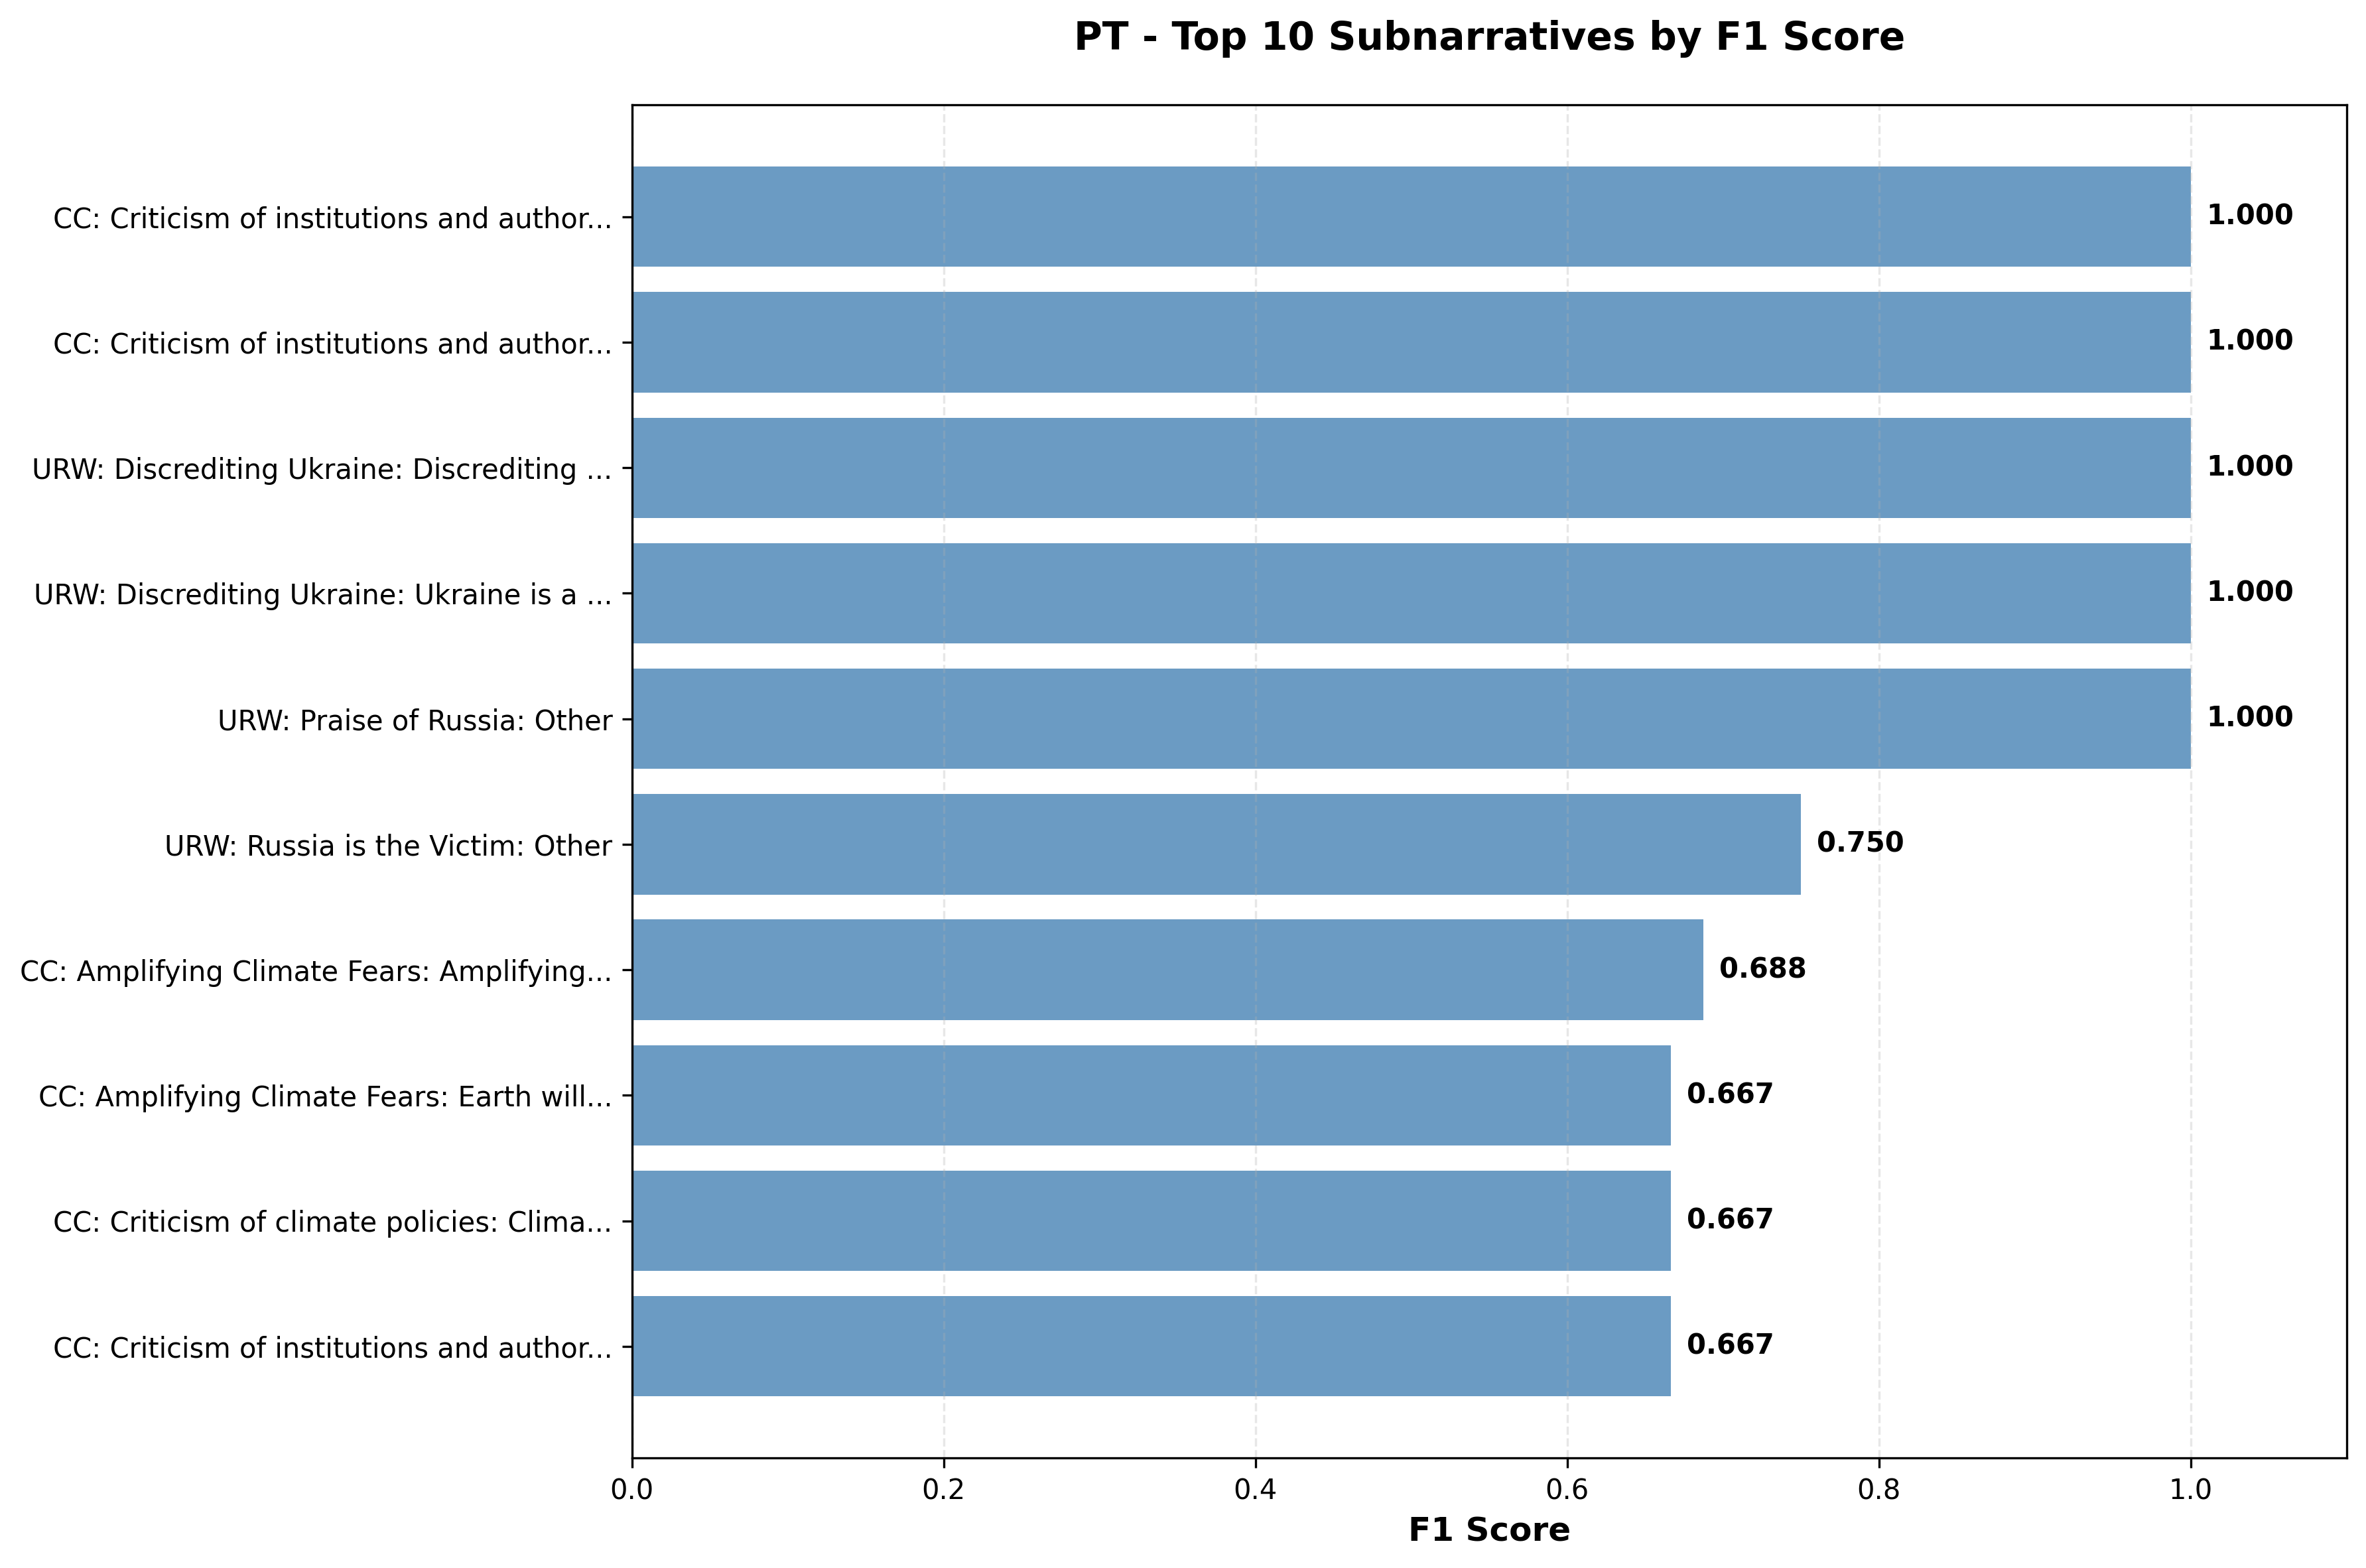
\includegraphics[width=\textwidth]{gemini25_flash_devset_evaluation/plots/PT_top_subnarratives_f1_scores.png}
        \caption{Portuguese subnarratives}
        \label{fig:pt-subnarratives}
    \end{subfigure}
    \hfill
    \begin{subfigure}[b]{0.48\textwidth}
        \centering
        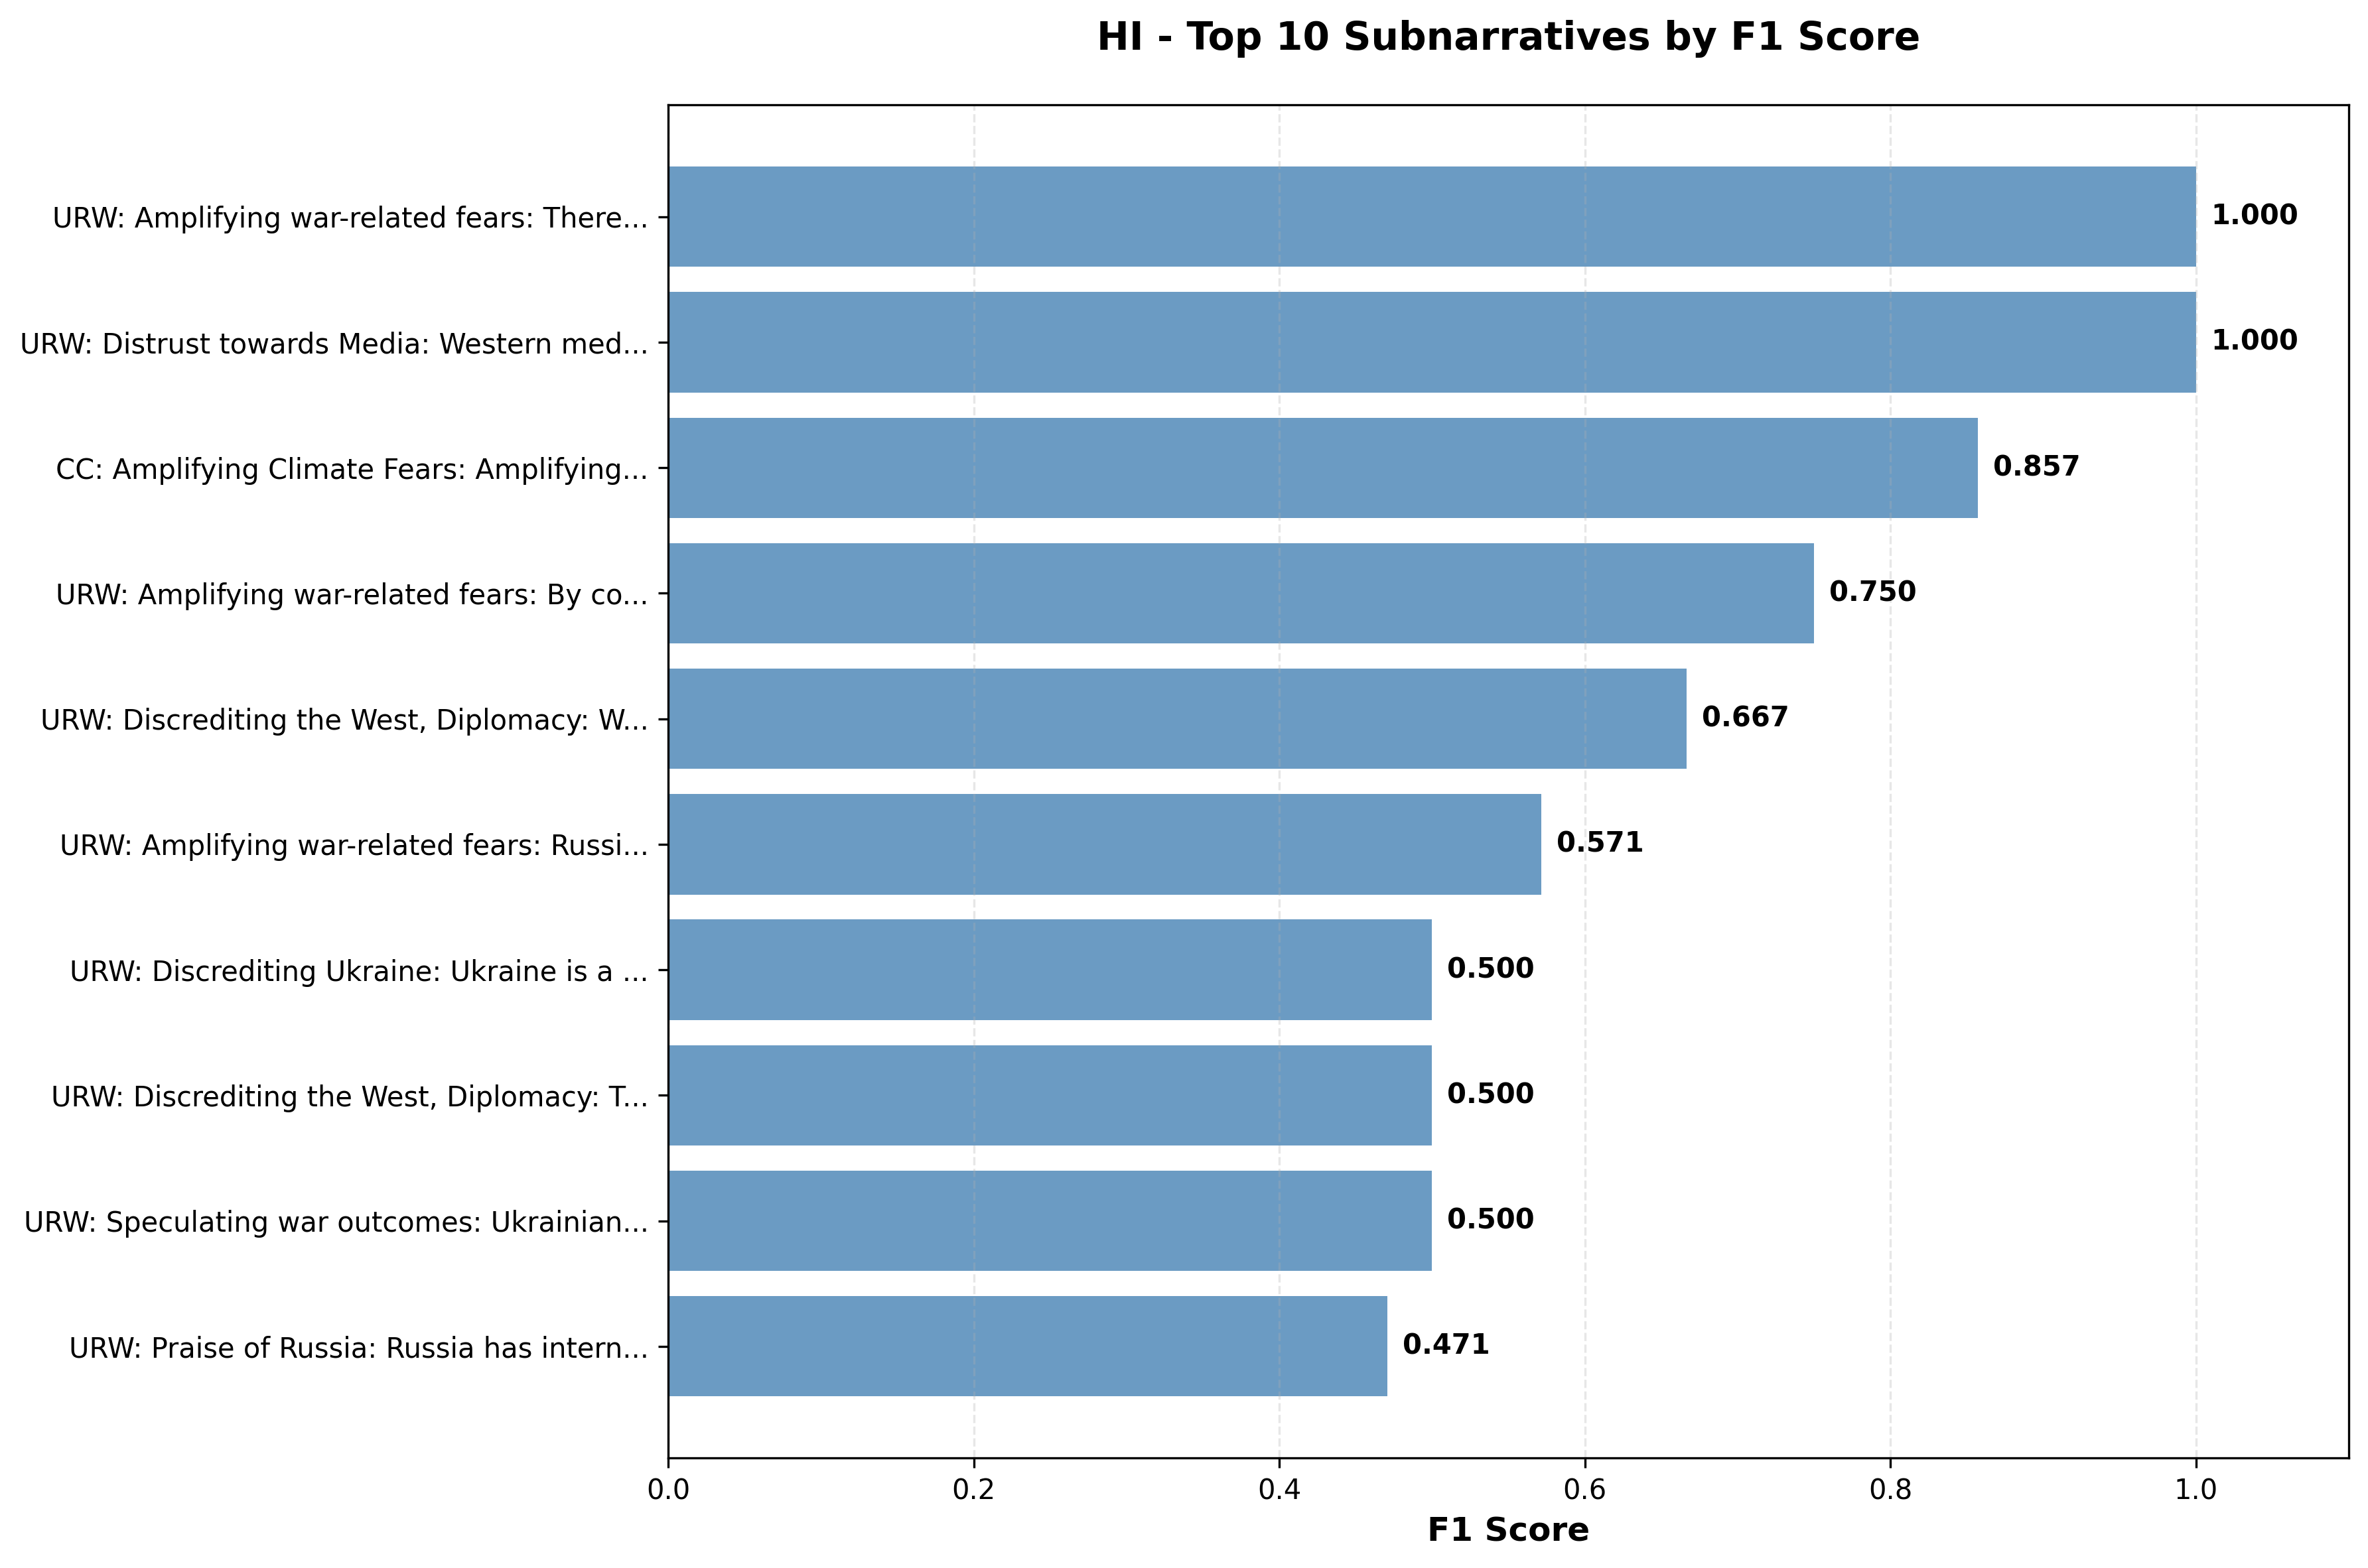
\includegraphics[width=\textwidth]{gemini25_flash_devset_evaluation/plots/HI_top_subnarratives_f1_scores.png}
        \caption{Hindi subnarratives}
        \label{fig:hi-subnarratives}
    \end{subfigure}
    \caption{Subnarrative performance comparison between the best (Portuguese) and most challenging (Hindi) languages. Portuguese maintains strong performance even at fine-grained levels, while Hindi shows the characteristic challenges of low-resource language processing in nuanced classification tasks.}
    \label{fig:subnarrative-performance-by-language}
\end{figure}

\subsubsection{Portuguese maintains fine-grained excellence}

Portuguese achieves remarkable performance even at the subnarrative level:
\begin{itemize}
    \item Multiple perfect classifications (F1 = 1.000) across diverse categories
    \item \textbf{CC: Amplifying Climate Fears: Amplifying existing fears}: F1 = 0.688 with strong recall (0.786)
    \item Consistent high precision across categories, indicating effective false positive control
\end{itemize}

\subsubsection{Hindi subnarrative challenges}

Hindi reveals systematic challenges at the subnarrative level:
\begin{itemize}
    \item Best performance: \textbf{URW: Amplifying war-related fears: Real possibility of nuclear war} (F1 = 1.000)
    \item \textbf{CC: Amplifying Climate Fears: Amplifying existing fears}: F1 = 0.857
    \item Significant performance degradation on most categories, with many achieving F1 < 0.500
\end{itemize}

\subsection{Comparative analysis with baseline architectures}

The actor-critique pipeline demonstrates substantial improvements over the transformer baseline:

\paragraph{Hierarchical error mitigation.} The 19.4\% average performance gap between narratives and subnarratives represents a significant improvement over the transformer baseline's 60\% gap, validating the effectiveness of the critique validation mechanism.

\paragraph{Multilingual consistency.} Portuguese performance (F1 Samples: 0.7489 for narratives) substantially exceeds the transformer baseline's best language performance, while maintaining strong cross-linguistic consistency.

\paragraph{Precision enhancement.} The frequent achievement of perfect precision scores (1.000) across multiple categories demonstrates the critique mechanism's effectiveness in reducing false positives.

\subsection{Key insights and architectural implications}

\paragraph{Validation mechanism effectiveness.} The actor-critique pipeline successfully addresses many error propagation issues identified in hierarchical classification, though challenges remain with rare categories and cultural nuances.

\paragraph{Language-specific optimization potential.} The substantial performance variations across languages (PT: 0.7489 vs HI: 0.4715) suggest opportunities for language-specific prompt engineering and cultural context integration.

\paragraph{Scalability considerations.} While effective, the two-stage architecture introduces computational overhead, particularly relevant for production deployment across multiple languages.

The actor-critique pipeline establishes a strong foundation for zero-shot multilingual narrative classification, demonstrating that carefully designed validation mechanisms can significantly improve hierarchical classification performance while maintaining the advantages of the zero-shot paradigm.
